\begin{frame}{Thực nghiệm: Dữ liệu và phương pháp}
    \begin{itemize}
        \item Tập dữ liệu: MNIST, CIFAR10, ImageNet
        \begin{itemize}
            \item MNIST và CIFAR10 được huấn luyện trên mô hình DNN bởi Carlini và Wagner
            % \begin{itemize}
            %     \item Lấy ngẫu nhiên 1000 ảnh test đã được phân loại đúng để tấn công
            % \end{itemize}
            \item ImageNet sử dụng mô hình InceptionV3
            % \begin{itemize}
            %     \item Chọn 100 ảnh đã được phân loại đúng và 9 lớp khác để tấn công
            % \end{itemize}
        \end{itemize}
        \item Phương pháp tấn công:
        \begin{itemize}
            \item EAD
            \item C\&W
            \item FGM
            \item I-FGM
        \end{itemize}
        \item Phần cứng: Intel E5-2690 v3 CPU, 40 GB RAM, NVIDIA K80 GPU
    \end{itemize}
\end{frame}

\begin{frame}{Thực nghiệm: Độ đo}
    \begin{itemize}
        \item ASR: Tỉ lệ tấn công thành công
        \item $L_1$, $L_2$ và $L_{\infty}$: Các khoảng cách giữa mẫu đối nghịch và ảnh gốc
    \end{itemize}
\end{frame}

\begin{frame}{Thực nghiệm: Các trường hợp quan tâm}
    \begin{itemize}
        \item \textbf{Trường hợp tốt nhất (best case):} tấn công dễ nhất về phương diện nhiễu, trong số các tấn công nhắm tới tất cả các lớp sai nhãn.
        \item \textbf{Trường hợp trung bình (average case):} tấn công nhắm ngẫu nhiên vào 1 lớp sai nhãn.
        \item \textbf{Trường hợp xấu nhất (worst case):} tấn công khó nhất về phương diện nhiễu, trong số những tấn công nhắm tới tất cả các lớp sai nhãn.
    \end{itemize}
\end{frame}

\begin{frame}{Thực nghiệm: Độ nhạy}
    \begin{figure}
        \centering
        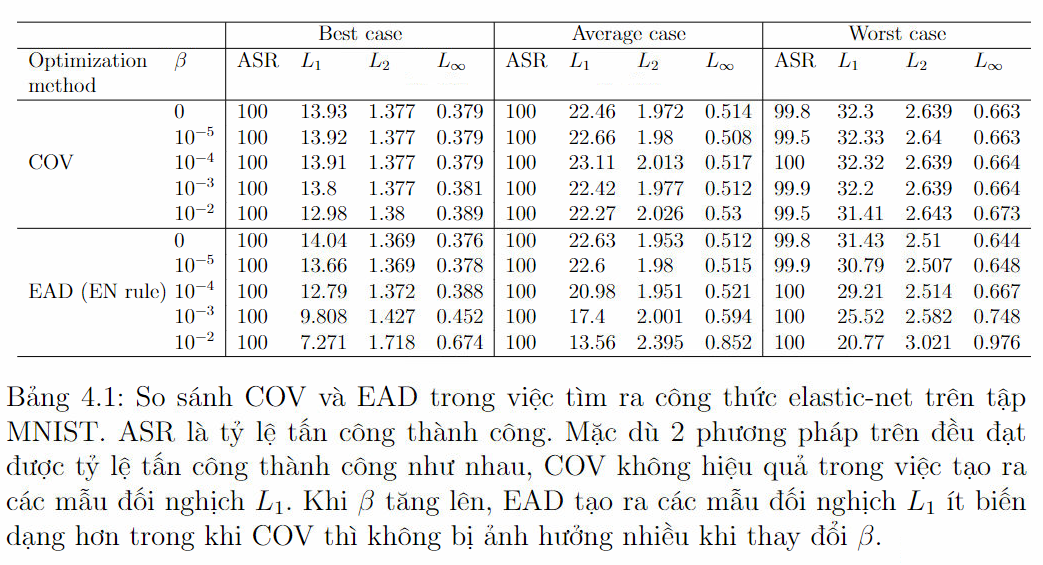
\includegraphics[scale=0.5]{images/tab_4_1.png}
    \end{figure}
\end{frame}

\begin{frame}{Thực nghiệm: Luật quyết định}
    \begin{figure}[H] % places figure environment here   
        \centering % Centers Graphic
        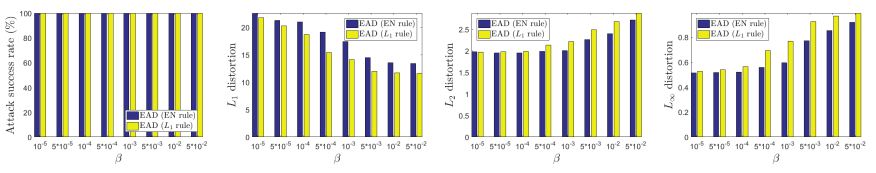
\includegraphics[width=1\textwidth]{images/fig_02.png} 
        \caption{So sánh luật quyết định EN và $L_1$ trong EAD trên tập MNIST với nhiều tham số hiệu chỉnh $L_1$ $\beta$ (trường hợp trung bình). So sánh với luật chọn EN tại cùng giá trị $\beta$ thì luật chọn $L_1$ thu được các mẫu ít nhiễu $L_1$ hơn, nhưng đổi lại có thể bị nhiễu $L_2$, $L_{\infty}$ nhiều hơn.}% Creates caption underneath graph
        \label{fig:fg_02}
    \end{figure}
\end{frame}

\begin{frame}{Thực nghiệm: ASR, nhiễu trên MNIST, CIFAR10, ImageNet}
    \begin{figure}
        \centering
        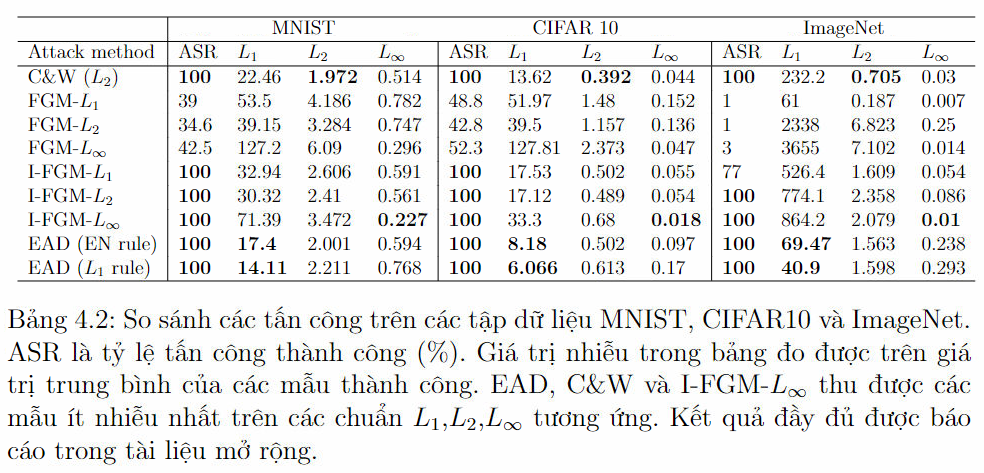
\includegraphics[scale=0.55]{images/tab_4_2.png}
    \end{figure}
\end{frame}

\begin{frame}{Thực nghiệm: Phá vỡ chắt lọc phòng thủ}
    \begin{figure}[H] % places figure environment here   
        \centering % Centers Graphic
        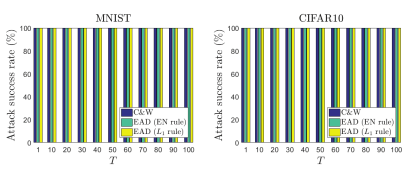
\includegraphics[width=0.6\textwidth]{images/fig_3.png} 
        \caption{ASR (trường hợp trung bình) của C\&W và EAD trên tập MNIST và CIFAR10 với các tham số nhiệt $T$ khác nhau cho chắt lọc phòng thủ. Cả 2 phương pháp đều phá vỡ thành công chắt lọc phòng thủ.} % Creates caption  % Creates caption underneath graph
        \label{fig:fg_03}
    \end{figure}
\end{frame}

\begin{frame}{Thực nghiệm: Chuyển giao tấn công}
    \begin{figure}[H] % places figure environment here   
        \centering % Centers Graphic
        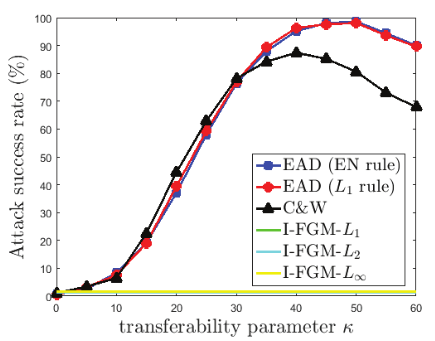
\includegraphics[width=0.5\textwidth]{images/fig_04.png} 
        \caption{Khả năng chuyển giao tấn công (trường hợp trung bình) từ mạng không phòng thủ sang mạng chắt lọc phòng thủ  trên tập dữ liệu MNIST với các tham số $\kappa$ khác nhau. EAD có thể đạt ASR gần $99\%$ khi $\kappa = 50$, trong khi ASR lớn nhất của C\&W là gần $88\%$ khi $\kappa=40$.} % Creates caption  % Creates caption underneath graph
        \label{fig:fg_04}
    \end{figure}
\end{frame}

\begin{frame}{Thực nghiệm: Huấn luyện đối nghịch bổ sung}
    \begin{figure}
        \centering
        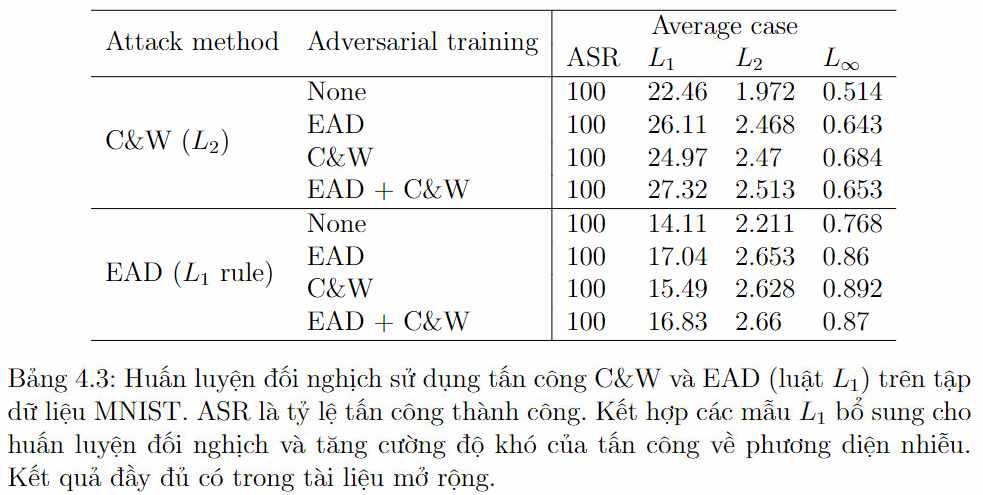
\includegraphics[scale=0.55]{images/tab_4_3.png}
    \end{figure}
\end{frame}

